\section{Problem Definition}
\label{sec:prob}
\newtheorem{definition}{Definition}


In this part, we will describe our problem model firstly, then the formal definition of the problem will be given.
In the last of this part, we will discuss our problem theoretically and analyze the problem from various aspects.

\begin{table}[htp]
\caption{the meaning of symbols}\label{analogy}
\centering
\begin{tabular}{|l|l|}
  \hline
  % after \\: \hline or \cline{col1-col2} \cline{col3-col4} ...
  \hline
  $n_i$ & \footnotesize{the node i}\\
  $v_i$ & \footnotesize{the speed of node i}\\
  $T_{ik}$ & \footnotesize{the time of node i's $k$th contact}\\
  $C_{ik}$ & \footnotesize{the node i's $k$th contact}\\
  $L_{ik}$ & \footnotesize{the possible location of node i's $k$th contact}\\
  $S_{ij}$ & \footnotesize{the distance between two contact nodes i and j in one contact}\\
  \hline
\end{tabular}
\end{table}

We define a map $M$ as a graph $(V,E)$, where $V$ is a set of junctions each with geometric coordinates $(x,~ y)$,
and $E$ is a set of straight road segment. Note that a curved road can be approximated by a sequence of straight road
segment. Let a set of nodes $N$ move on the edges of the map at constant speed.
Let the trace of node $i$ be a function of locations on time $l_i(t)$.
Let a {\em contact} between node $i$ and $j$ be a 4-tuple: $(i, j, t_{in}, t_{out})$
where $t_{in}$ is the time $i$ and $j$ encounter each other, and $t_{out}$ is the time
$i$ and $j$ depart. Further, a {\em contact history} is a set of contacts.
Given the set of traces of $N$, we can {\em induce} all the contacts by solving equations

\begin{equation}
||l_i(t)-l_j(t)|| \leq d
\label{eqn:contact}
\end{equation}

\noindent
for all pairs of traces by node $i$ and $j$, where $d$ is the range in which two nodes are considered in contact.
For simplicity, we assume $d=0$ in the rest of this paper. (\ref{eqn:contact}) can be computed
in $O(|N|^2|V|^2)$ time.


%%%%%%%%%%%%%%%%%%%%%
%There are $N$ nodes moving in the map,
%the movement of each node is confined within the roadways and the speed $v_i$ of the node $n_i$ is uniform, $n_i$ denotes the node ID.
%Let $L_i(t)=(x_i(t),y_i(t))$ be the coordinates of node i, and $\exists e,e' \in E$, s.t. $L_{ik}$ and $L_{jm}$ are on $e,e'$ respectively.
%We consider two nodes have a contact if they come into the communication range $d$, and each of them will record a contact history.
%Each contact history is recorded as $C_{ik}$=\{$T_{ik},n_i,n_j$\}, where $k$ represents that it is the recorder's $k$th record, $T_{ik}$ is the contact time recorded by $n_i$ who is the recorder and $n_j$ is the contact node.
%We assume that these contact histories are obtained and sorted by time order.
%We define a trace for node $i$ as $\{L_{i0}(T_0),L_{i1}(T_{i1}),...,L_{ik}(T_{ik}),...\}$, where $L_{ik}(T_{ik})$  $k$ is the $k$th location at the $k$th contact, each location $L_{ik}$ corresponds to a sequence of junctions which generates the location.
%Since in a contact event at time $T$, corresponding to node $n_i$'s location $L_{ik}(T)=(x_i(T),y_i(T))$, there must exist an another node $n_j$ whose location $L_{jm}(T)=(x_j(T),y_j(T))$, so that $L_{ik}$ and $L_{jm}$ satisfy the contact condition:
%\begin{displaymath}\label{equ:con}
%  (x_i(T)-x_j(T))^2+(y_i(T)-y_j(T))^2\leq d^2
%\end{displaymath}
%, where $d$ is the communication range.
%%%%%%%%%%%%%%%%%%%%%%%%

 We define the Trace Inference Problem(TIP) as
 \begin{definition}
 \textbf{Trace Inference Problem(TIP)} Given a map $M$, a set of moving nodes $N$, their speeds $\{v_i\}$, their initial locations $\{l_i(0)\}$, and a contact history $H$,
 find the traces of $N$ whose induced contact times $H_{ind} = H$ .
 \end{definition}

\subsection{Baseline Approach}
Suppose $i$ and $j$ contact at time $t$, their previous contact time are $t_i$ and $t_j$ respectively, thus the moving distance of $i$ and $j$ is $s_i=v_i(t-t_i),s_j=v_j(t-t_j)$. Intuitively, we consider this problem through solving each contact, given the initial location and the first contact, we could infer some possible locations of two contact nodes at $t$, we define possible location and possible initial location as
\begin{definition}
A possible location $l_i(t_i)$ is the location after last contact time $t_i$, and the inferred possible locations of a particular node before its next contact are its possible initial locations in its next contact from which we begin to search.
\end{definition}
As showed in Fig.\ref{fig:des}, we have a contact history of A and B, and we assume that we have the initial locations of them so that we could infer their traces based on the locations and contact information. Firstly through enumerating all the possible paths, we find out 5 possible traces of A from its initial location to A1, A2, A3, A4 and A5 respectively . On the other hand, we could also enumerate all the B's possible traces, but we note that as B could get to location B2 through two different paths, thus B only has 5 possible locations (B1,B2,B3,B4 and B5) corresponding to 6 possible traces. Based on the enumeration results of two nodes, we can justify which pair of possible locations satisfy the contact condition, then we exclude those traces whose possible location has no partner. So we find out all possible locations of A and B, as A1-A4 and B1-B3 (B2 corresponds to A2 and A3 respectively), then we record these possible traces for A, B and we take A1-A4 as the possible initial locations for A in its next contact to search, the same with B1-B3. When we get a new contact history of B and C, we repeat aforementioned process, but here we should enumerate B's possible traces from all its initial locations B1-B3 generated from last contact. Furthermore, not only we could exclude the impossible locations such as B2' and C2, but also could exclude B2 and B3 which can't be excluded in the last contact.







%Initially we consider the enumerating search approaches to solve this problem.
%We focus on an individual node and attempt to find out all its possible paths based on each of its contact history records.
%But we find that its possible paths will diverge into numerous possible traces, which will make our work more difficult.
%When we search for a possible trace, any junction on the path will increase the entropy of the possible solution, which means the more junctions on the possible path, the more uncertainty in our solutions.
%Otherwise each contact history will constrain our solutions in a reasonable range, which means the solutions must satisfy the contact condition, while reducing the complexity of our problems.
%We take those new possible locations generated from the last contact histories as the new possible initial locations in the next contact histories.
%Therefore we decompose our Trace Inference Problem into numbers of small Trace Inference Problem.
%In a small Trace Inference Problem, when given the possible initial locations and the next contact history, we infer the next possible locations for both of the contact nodes.



%\begin{figure}[th]
%\label{fig:des}
%\centering
%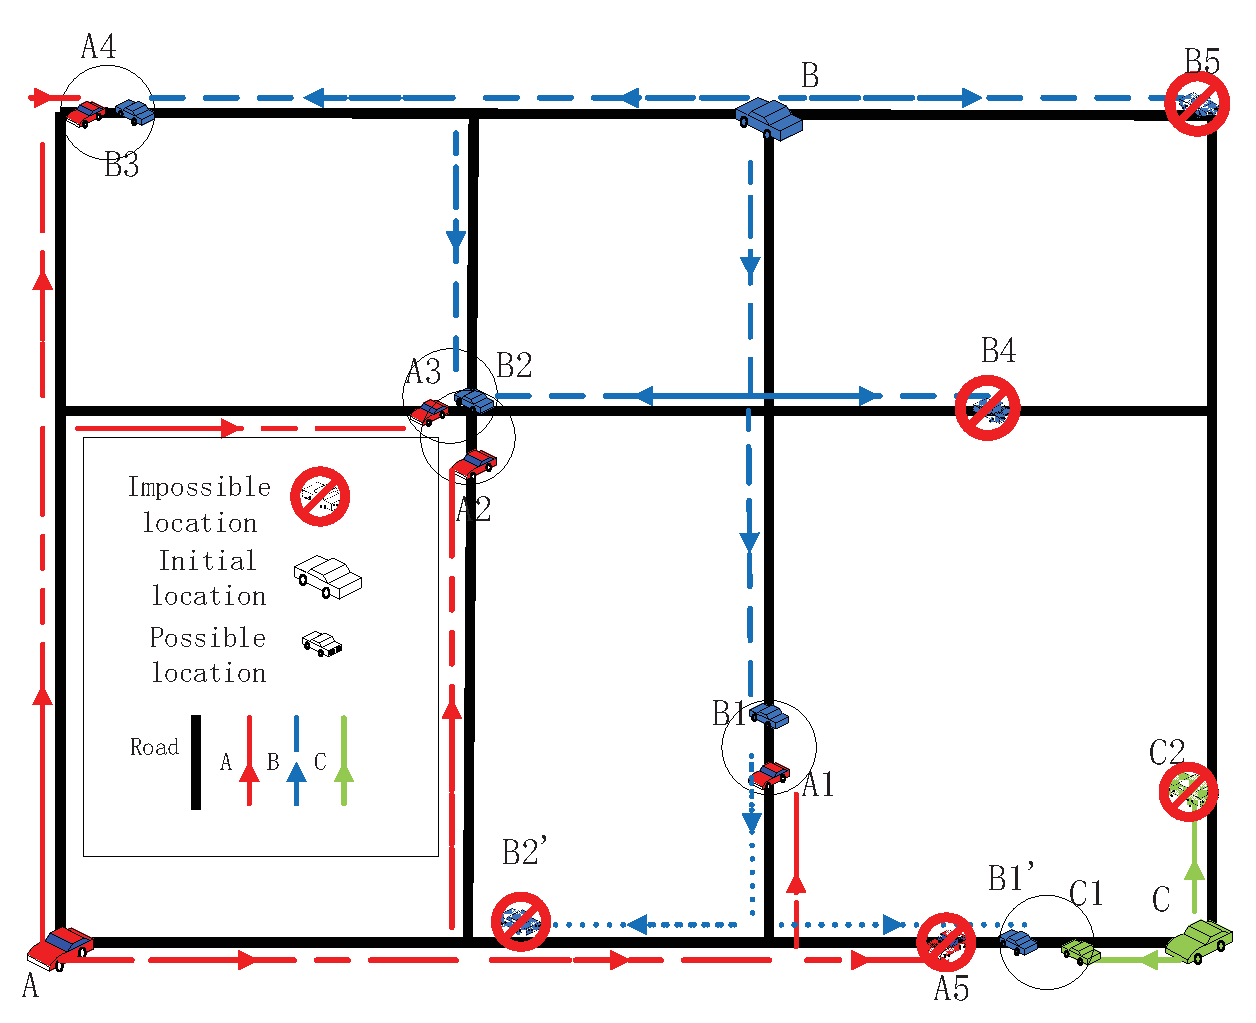
\epsfig{file=11.eps, width=0.9\columnwidth}
%\caption{A simple example of trace inference based on one contact history}
%\end{figure}

 \begin{definition}
 The searching entropy $H(l_i(.))$ of a node $i$ from its last contact time $t'$ to this contact time $t$ is the entropy of all its possible searching traces $\{l_i(.)\}_{t'-t}$, which is expressed as
 \begin{displaymath}
 H_{t'-t}(l_i(.))=\sum p(l_i(.)) \log p(l_i(.))
 \end{displaymath}
 ,where $p(l_i(.))$ is the searching probability of the trace $l_i(.)$
 \end{definition}

For example, in Fig.\ref{fig:des}, we search 5 possible traces of A from its initial location. Since we assume that searching probability at each junction is uniform, thus the probabilities of traces from A to A2,A3,A4 are all $\frac{1}{4}$, then $H(A)=-\sum_1^4 \frac{1}{4}\log\frac{1}{4}=\log 4$; B could reach B1-B3 three places, but since B could reach B2 through two different ways, thus $p(B2)=\frac{1}{4}+\frac{1}{4}=\frac{1}{2}$, then $H(B)=-(\frac{1}{4}\log\frac{1}{4}+\frac{1}{2}\log\frac{1}{2}+\frac{1}{4}\log\frac{1}{4})=\frac{3}{2} \log 2$.

\textbf{Longest Path Problem}. Given a weighted graph $G=(V,~E)$
two distinguished vertices $s,t /in V$ and a positive integer $c$,
is there a \emph{simple} path in $G$ from $s$ to $t$ of length $c$ or more?

\textbf{Lemma} \textbf{Longest Path Problem} is an NP-complete problem \cite{NP-complete}.

\textbf{Theory} \textbf{Trace Inference Problem} is a an NP-complete problem.

{\bf Proof:}\\
Since trace inference is based on the contact histories and initial locations, and through each of contact histories, we could get one or more new possible locations at the contact moment, thus \textbf{Trace Inference Problem} can be divided into numbers of small problems which are based on a single contact history and the node's last possible locations to infer the traces. Since the number of these small problems is determined as $\sum_{i=1}^N {K_i}$ (the number of contact histories), we just need to prove that the small problem of \textbf{Trace Inference Problem} is an NP-complete problem.

The small problem of \textbf{Trace Inference Problem} can be described as: Given some possible initial locations of two contact nodes and the contact history, can we find out all the possible traces that satisfy the distance between two possible initial locations lies in $[S_{ij},~S_{ij}+d]$, where $S_{ij}=s_{ik}+s_{jm}$ is the movement distance of two contact nodes in a contact history, $d$ is the contact range.

The first step in proof is to show that the small problem of \textbf{Trace Inference Problem} is in the NP.
It is obvious that there is a nondeterministic algorithm can start by guessing two paths of two contact nodes, then verifies whether this two paths could make two nodes contacted with each other at the contact time.

The next step is to show that \textbf{Longest Path} can be reduced to the small problem of \textbf{Trace Inference} in polynomial time, i.e.,
\begin{displaymath}
\textbf{Longest Path} \propto_{poly} \textbf{the small problem of Trace Inference Problem}.
\end{displaymath}

As the graph is in a limited area, thus the distance between two nodes must be finite, we assume that the longest distance between two nodes is $d_{max}$, then the range in \textbf{longest Path} from $[c,\infty)$ turns to be $[c,~d_{max}]$. So we set $c=\lfloor S_{ij} \rfloor$, $d_{nax}=\lfloor d+c \rfloor$, then \textbf{Longest Path} is reduced to be the small problem of \textbf{Trace Inference}.





%We will show in this paper that it is possible to automatically infer one or more
%victims' complete or partial movement traces given only their
%initial locations, their average speed, their complete contact histories,
%and a map of the area where the contacts occured.
%This technique can be deployed both indoors and outdoors, so long
%as the map with accurate coordinate information is available.

